\section{Models}
%This model was tested 
%with a benchmark instance of 30 points, 
%which sets $V$ and $W$ are the same.
%For values of $p = 1,\ldots,7$
%the optimal solution was found in less than one minute.
%
%For other benchmark instances
%was impossible to find the solution
%because they have more than 300 points,
%and the proposed model grows to over one million variables.
%  For some large instances ($n = 50$ , $m = 30$)%

These test were evaluated in
a Lanix Spine BW Processor Intel Xenon,
CPU E5-2867W, 3.10 GHz.
With operative system Ubuntu 14.04.3 LTS
The models were solved with CPLEX 12.6.0.0,
and they were coded in C++.

Different random instances were generated
to validate the proposed formulations.
For $n = 100$ we created 8 instances with $m = 20,30,\ldots,100$,
and they were tested with different values of $p$ from 5 to $\frac{m}{2}$,
shown in the following table \ref{tab:tests}.
\begin{table}
  \centering
  \begin{tabular}{|c|c|c|}\hline
    n & m & p \\ \hline
    100 & 20 & 5-10 \\
    100 & 30 & 5-15 \\
    100 & 40 & 5-20 \\
    100 & 50 & 5-25 \\
    100 & 60 & 5-30 \\
    100 & 70 & 5-35 \\
    100 & 80 & 5-40 \\
    100 & 90 & 5-45 \\
    100 & 100 & 5-50 \\
    \hline
  \end{tabular}
  \caption{Instances to test models}
  \label{tab:tests}
\end{table}

Model A was solved to optimality only when $p < 25$,
in an average time of 217 seconds.
for the rest of the values of $p$, 
no factible solution was found for $65\%$ of the test cases
in less than 20 minutes,
for the rest test cases,
an average gap of $27\%$ was obtained.

Model B was evaluated
with the same combinations of $n,m,p$
and $\ell$ from $1,\ldots,p$.
For almost all cases,
model B was solved to optimality
in less than a minute for each case.
\begin{figure}[!ht]
  \centering
  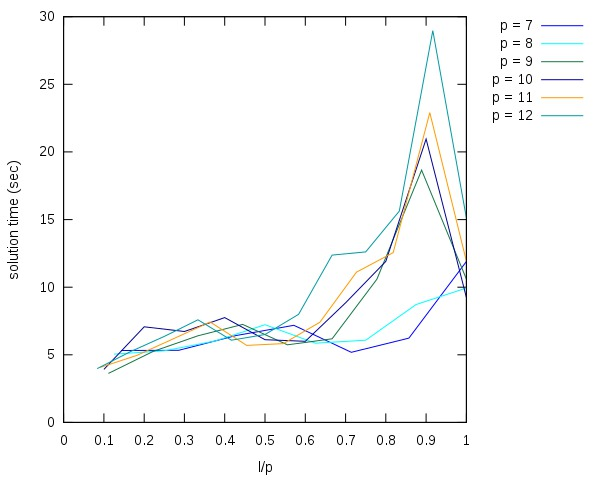
\includegraphics[scale=0.6]{graph_01}
  \caption{Solution times versus $\ell$ between $p$}
\end{figure}

When the value of $\ell$ 
is close to $p$
model resolution takes longer
and in some cases
optimal is not achieved.
\begin{figure}[!ht]
  \centering
  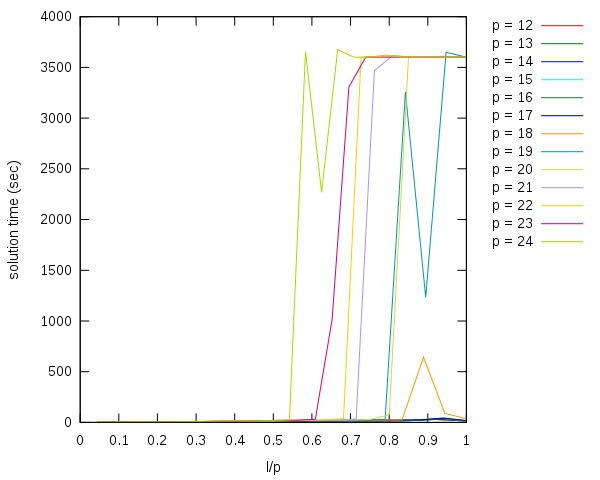
\includegraphics[scale=0.35]{graph_02}
  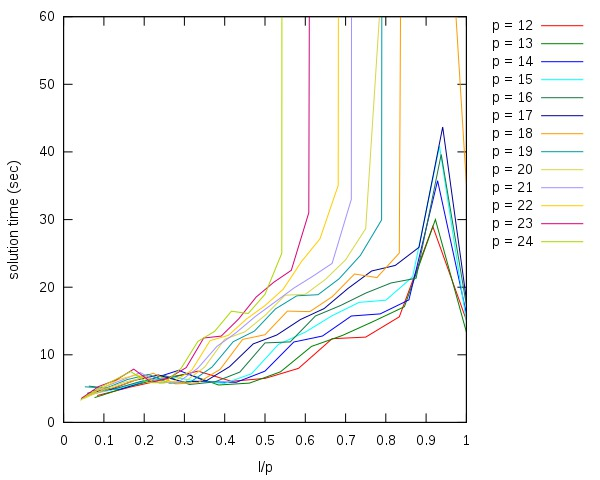
\includegraphics[scale=0.35]{graph_03}
  \caption{Solution times versus $\ell$ between $p$}
\end{figure}

However,
it can be seen
that for different values of $\ell$
the solutions obtained are the same.

\begin{figure}[!ht]
  \centering
  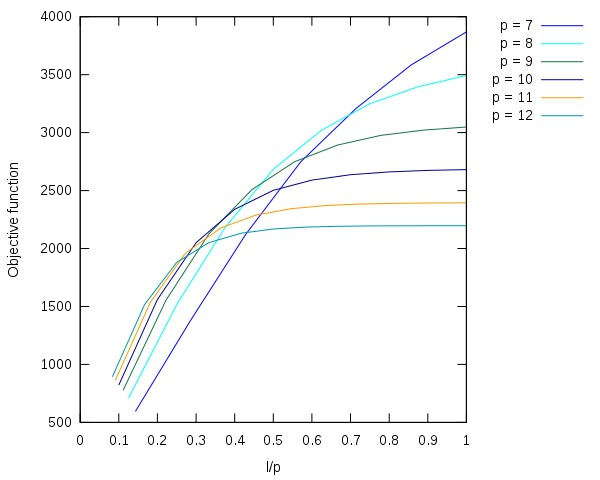
\includegraphics[scale=0.35]{graph_04}
  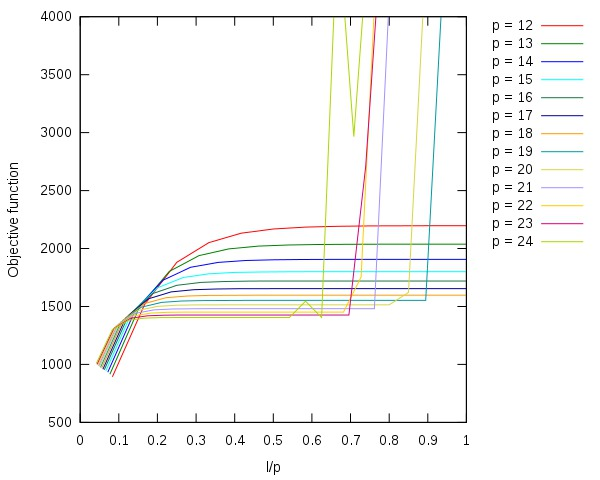
\includegraphics[scale=0.35]{graph_05}
\end{figure}
